
%%%%%%%%%%%%%%%%%%%%%%%%%%%%%%%%%%%%%%%%%%%%%%%%%%%%%%%%%%%%%%%%%%%%%%%%%%%%%%%%%%%%%%%
% Denna fil kompileras (pdflatex designspec.tex)
% Inga ändringar bör behöva göras
% Saknar din installation bibliotek? Installera dem eller skrik på dokumentansvarig.
%%%%%%%%%%%%%%%%%%%%%%%%%%%%%%%%%%%%%%%%%%%%%%%%%%%%%%%%%%%%%%%%%%%%%%%%%%%%%%%%%%%%%%%

% Document props and library inclusions
\documentclass[10pt,a4paper]{report} 
\usepackage[utf8]{inputenc} 
\usepackage[english]{babel}
\usepackage{mathtools,tikz,textcomp,fixltx2e,color,fullpage,graphicx,afterpage,float,parskip,xfrac,gensymb,titlesec,etoolbox,pdfpages,hyperref}
\usetikzlibrary{calc,matrix,positioning,arrows,shapes,trees,plotmarks,decorations.markings}
\usepackage[font={small,it}]{caption}
\usepackage[europeancurrents,europeanvoltages,europeanresistors,europeaninductors,smartlabels]{circuitikz}
\usepackage[font={small,it}]{caption} %% Italics in captions

\setcounter{secnumdepth}{2} % Levels enumerated

% PDF props
\hypersetup{
  bookmarks=true,              % show bookmarks bar?
  bookmarkstype=toc,
  bookmarksopenlevel=\maxdimen
  unicode=true,                % non-Latin characters in Acrobat’s bookmarks
  pdftoolbar=true,             % show Acrobat’s toolbar?
  pdfmenubar=true,             % show Acrobat’s menu?
  pdffitwindow=false,          % window fit to page when opened
  pdfstartview={FitH},         % fits the width of the page to the window
  pdftitle={Design Specification},         % title
  pdfauthor={Petersson, Oscar}, % author
  pdfsubject={TSIU03},          % subject of the document
  pdfkeywords={TSIU03}          % list of keywords
  pdfnewwindow=true,           % links in new window
  hidelinks,                   % hide links (removing color and border)
  linktocpage=true,
  linktoc=all,                 % parts of TOC made into links
  pdfdisplaydoctitle=true      %display document title instead of file name in title bar
}
\urlstyle{same}

\graphicspath{{./fig/}} % including pictures from here

%% First Page Information
\author{Niklas Blomqvist, Philip Johansson, Matteus Laurent, Johan Levinsson, Oscar Petersson, Erik Peyronson}
\title{Group 41 - Design Specification}
\date{\today}
\newcommand{\course}{System Design - Project, HT15}
\newcommand{\coursenumber}{TSIU03, Linköpings universitet}
\newcommand{\programme}{Högskoleingenjörsutbildning i datateknik, 180 hp}
\newcommand{\examiner}{Petter Källström}
\newcommand{\institution}{Department of Electrical Engineering (ISY)}
\newcommand{\reptype}{Design Specification}

%\newcommand{\includelogo}{
\includegraphics[width=48 mm]{LiTH_sigill_sv.pdf}\makeatletter\begin{center}\vskip 4.5cm}
\newcommand{\excludelogo}{\makeatletter\begin{center}~\vfill}

%% Proper Chapter Head
\makeatletter
\renewcommand{\@makechapterhead}[1]{%
  \vspace*{50 pt}%
          {\setlength{\parindent}{0pt} \raggedright \normalfont
            \bfseries\Huge
            \ifnum \value{secnumdepth}>1
            \if@mainmatter\thechapter.\ \fi%
            \fi
            #1\par\nobreak\vspace{40 pt}}}
\makeatother

\begin{document}

\pagestyle{empty}
%\includelogo
 \excludelogo
  \Large{\@author}\vskip .3cm
  \textbf{\LARGE{\@title}}\vskip .2cm
  \large{\programme}
  \vfill
\end{center}
\reptype{} - \@date\hfill Supervisor:\\
\textbf{\course}\hfill\examiner\\
\coursenumber\hfill\institution
\makeatother
\newpage

%% Table of Contents
\addtocontents{toc}{\protect\hypertarget{toc}{}}
\tableofcontents\label{sec:toc}
\addtocontents{toc}{\protect\thispagestyle{empty}}
\cleardoublepage


%\chapter{Vad dokumentet ska innehålla:} % Detta ska bort innan inskick
%The entire Design Spec should be 5-7 pages

\begin{itemize}
\item Now you are the engineers who receive the requirement specification. What you have to do is to propose a solution that fulfills the requirements of the system.
\item Contrary to the requirements specifications, now you have to think about HOW you are going to meet  the requirements.
\item The design specification must describe the entire system. Think about the main blocks that your system will have, the functionality of each block and the interaction between them, i.e., which information the have to send to each other. Explain the functionality of the blocks and their interaction from a signal processing point of view, i.e., how the audio, video, etc. are processed in each block and which infomation is transmitted between blocks. You can provide som equations to show the algorithms that are applied. Note that this is very different from providing the hardware interfaces between the blocks.
\item Later, think about the difficulties that you will find in hardware and the hardware limitations (timing, bandwidth, word length, etc.) and check that your design is viable. Some calculations may be necessary. For instance, if a requirrement says that the system must be able to delay the audio signal one second, you will probably think of using a memory in order to meet the requirement. Then you should make some calculations to check how big the memory must be and if it fits in the FPGA or if you need to use an external memory.
\item The design specification must be described from the system level. Please, avoid details that are not relevant at that level. Also, make sure that the person who reads the document can get a clear idea of the entire system.
\item As a result, the design specification must be a technical proposal that shows that you have analyzed the problem and found the difficulties that you will face, and provides a first approach to the solution. A good approach for writing the design specification is to present a block diagram of the system, provide a high-level description (at signal processing level) about the functionality of each block and how the blocks interact, and show which requirements present challenges and how you will solve them in hardware.
\end{itemize}

\section{Layoutstandarder}
Läs README:n i ../Projektrapport/ först och främst. Jag har strukturerat det hela genom att ha varje chapter och section i en fil med motsvarande namn, och nya borde inte behövas. Referera till bilder, avsnitt etc. på adekvat sätt med\texttt{\textbackslash{}ref} (ger kapitelnummer eller figurnummer) och \texttt{\textbackslash{}pageref} (ger sidnummer).
Hänvisningar inom parentes sätts ej kursivt, i löptext anges de enligt (ta gärna en titt i description.tex):
\begin{verbatim}
  \emph{<Typ> \ref{ref:name}: Name}
\end{verbatim}

Jag föreslår även att vi använder oss av \verb#\verb+name+# för att markera namn på moduler, signaler, etc.

Förhoppningsvis har ni vid det här laget bekantat er med min \LaTeX{}-guide, men har ni frågor är det bara att hojta. Använd gärna emacs för att redigera dokumenten då det har stöd för uppmärkning av \LaTeX{}-syntax.

Får jag igång SSH:n till burken därhemma via skolans burkar ska jag försöka hålla autokompileringen vid liv under dagen, men jag garanterar inget.
                 % och likaså denna rad

\chapter{Introduction}\label{ch:introduction}
\setcounter{page}{1}

%%Första sidan
\begin{frame}
	\frametitle{Introduction}
		\begin{itemize}
			\item Audio signal processing
			\item 	Signal level indicator	
			\item Our own flavor:
				\begin{itemize}
				\item Background image
				\item Graphic scales for L/R input/output channels
				\item Class-D amplifier
			\end{itemize}
		\end{itemize}
\end{frame}


%%Andra sidan
%\begin{frame}
%\frametitle{UI}
%	\begin{itemize}
%		\item Volume
%			\begin{itemize}
%				\item Eleven different stages, exclusive mute.
%			\end{itemize}
%		\item Balance
%		\begin{itemize}
%				\item Seventeen different stages.
%			\end{itemize}
%		\item Mute
%		\item Peak level indicator
%	\end{itemize}
%\end{frame}


%Bild över UI
%%Tredje sidan

\begin{frame}
	\frametitle{UI}
	  \begin{figure}[h]
    \centering 
    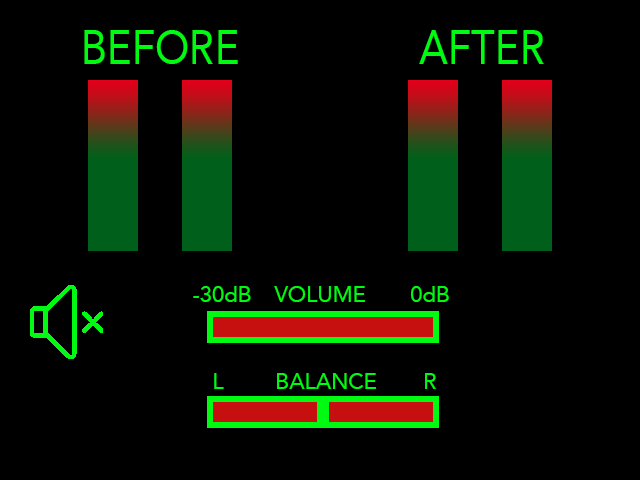
\includegraphics[scale=0.80]{UI2.png} 
       \label{UI}
  \end{figure}
\end{frame}




\chapter{System Level Description}\label{ch:description}
\emph{System Level Description (Block diagram + description of 1 to 2 pages).}

\emph{(Make sure that your description justifies how the Requirements of your system are met, especially those which are not obvious.)}

%% Remove the text above

This chapter will describe the system main blocks, the functionality of each of them, and the interaction between each block. Presented below (Figure \ref{fig:overview}) is a graphical overview over the system and its first layer of modules. A high resolution version is also included in \emph{Appendix \ref{app:overview}: System Overview}.

\begin{figure}[H]
  \centering
  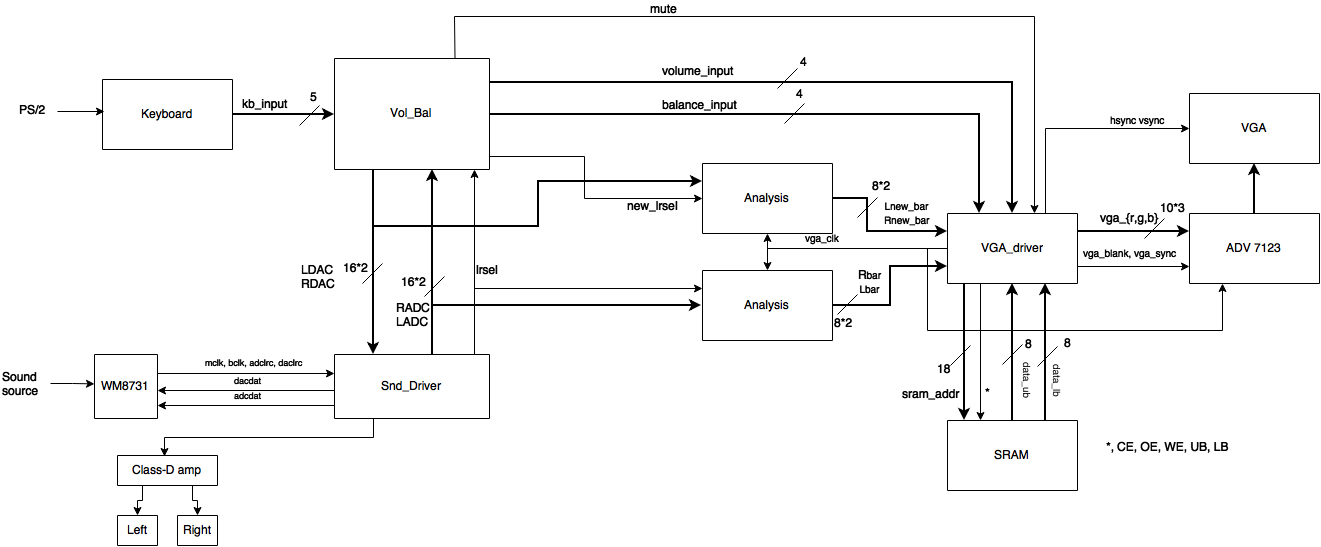
\includegraphics[scale=.18]{overview}
  \caption{A graphical overview of the system's first module layer.}
  \label{fig:overview}
\end{figure}

\section{Keyboard}\label{sec:keyboard}
The user interacts with the system through a PS/2-connected keyboard. The keyboard is then handled by the module \verb?Keyboard? which reads the scan codes, matches these against a \emph{one hot encoded} preset which makes up the \verb?kb_input? signal passed to \verb?Vol_Bal?.

The module inputs are \verb=PS2_DAT=, \verb=PS2_CLK=, \verb=clk= and \verb=rstn= which are used to shift in the scan code and compare the result with the preset, resulting in \verb=kb_input= --- a 2-bit unsigned value indicating if either of the arrow keys have been released. \verb=Vol_Bal= will then use this signal to adjust the volume and balance level. The Up/Down arrow keys controls the volume, and the Left/Right arrow keys controls the stereo channel balance.


\section{Snd\_Driver}\label{sec:snddriver}
The \verb?Snd_Driver? module is an audio signal coder/decoder. It translates the signal between a parallel format and a bit serial format. The parallel format is sent to the \verb?Vol_Bal? module which processes the sound and sends it to the class-D amplifier. The bit serial format is used by the WM8731 chip and the amplifier. This module will be a complete copy of the module used in \emph{Laboration 4}. In this case the module \verb?Vol_Bal? will replace and expand the \verb?Application? used in that laboration.

\begin{figure}[H]
  \centering
  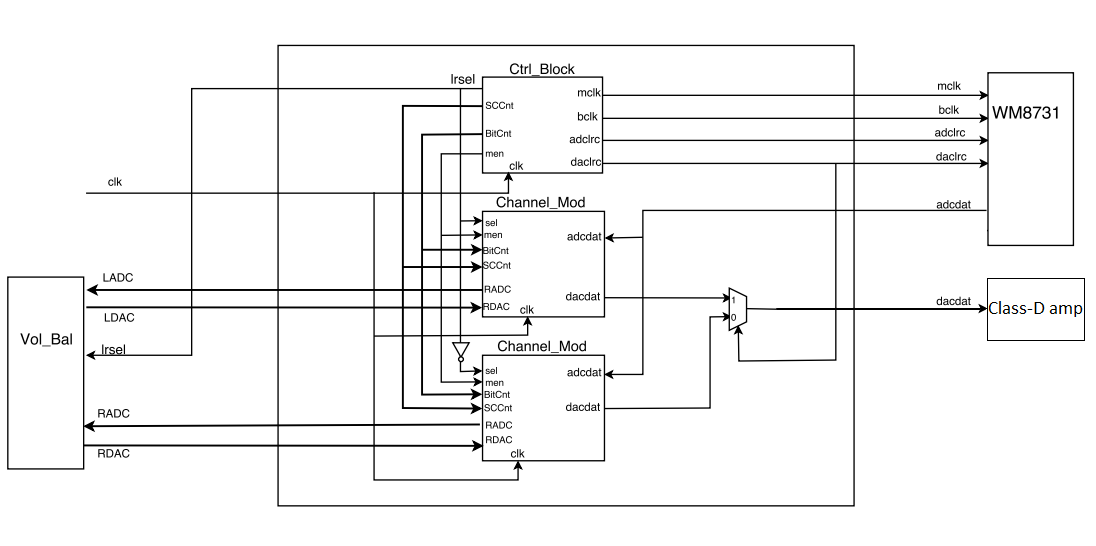
\includegraphics[scale=.40]{snddriver}
  \caption{The \texttt{Snd\_Driver} schematic, as seen in Lab 4, Audio Codec.}
  \label{fig:sndDriver}
\end{figure}


\section{Vol\_Bal}\label{sec:volbal}
The Volume/Balance module (\verb=Vol_Bal=) acts as the hub for processing incoming digital audio signals, forwarded from WM8731 via the \verb=Snd_Driver= module. As such, \verb=Vol_Bal= also keeps internal registers in the module \verb=Current_Vol_Bal= that holds volume (4-bit unsigned) and balance levels (4-bit signed), as well as a mute signal (std\_logic). These registers update via the one-hot coded input signal \verb=kb_input= applied by the \verb=Keyboard= module. Consequently, the values they hold are not only used as signals (\verb=i_volume_lvl=, \verb=i_balance_lvl=, \verb=i_mute=) for the internal submodule that process the \verb=LADC= and \verb=RADC= inputs, but also as module outputs connected to the \verb=VGA_Driver= so that they can be rendered on the screen.

\begin{figure}[h]
  \centering
  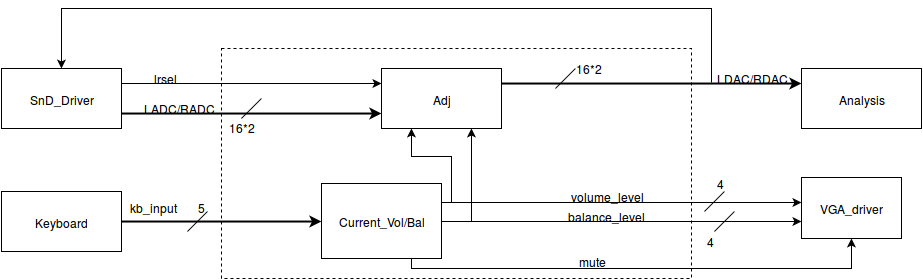
\includegraphics[width=16cm]{volbal}
  \caption{An overview of the Vol\_Bal module's internal workings.}
  \label{fig:vol_bal}
\end{figure}

The main function of the Volume/Balance module is to make requested adjustments to incoming values \verb=LADC= and \verb=RADC=, which represent measured amplitudes of the sound signal at distinct times. The sound will be adjusted for volume and balance by the functions:

\verb=   =$$A_{l\_new} = A_{l\_old} \cdot (1/\sqrt{2})^{n + m}\qquad\ ,\ m = 0\ for\ m < 0$$
\verb=   =$$A_{r\_new} = A_{r\_old} \cdot (1/\sqrt{2})^{n + |m|}\qquad,\ m = 0\ for\ m > 0\ ,$$

where $A$ is the amplitude, $n$ the volume level and $m$ the balance. \verb=lrsel= is used as a control signal for selecting the channel and the correct function. Resulting outputs \verb=LDAC= and \verb=RDAC= are forwarded to \verb=Snd_Driver= and to one instance of the \verb=Analysis= modules.

Ultimately, the user have the ability to digitally adjust the input sound by decreasing the volume in 3 dB decrements, down to -30 dB, and additionally regulate balance bias by further reducing volume by up to another 15 dB on a single left/right audio channel. There is also a mute function which is conveyed by \verb=kb_input=. When active, the register driving the \verb=mute= signal essentially blanks any $A_{new}$ values on the \verb=LDAC/RDAC= outputs.




\section{Analysis}\label{sec:analysis}
\begin{frame}
  \frametitle{Analysis}
	\begin{itemize}
		\item Analyzes incoming samples, low-pass filtering them.
		\item Output in form of a natural number, which determines the height of the bars.
		\item Updates in synd with vsync.
		\item Both left & right channel separately.
	\end{itemize}
\end{frame}

\begin{frame}
  \frametitle{Analysis}
	\begin{figure}[h]
		\centering
			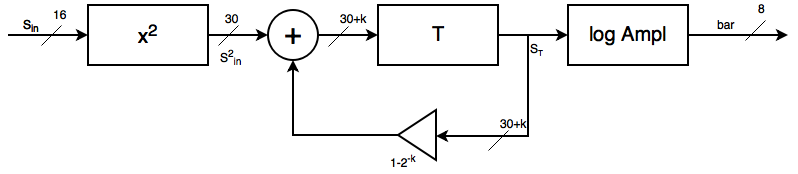
\includegraphics[width=16cm]{lowpass}
			\caption{The low-pass filter. $k$ is chosen by the approximation $\frac{1}{10}\mathrm{\ s} = 2^k\cdot\frac{1}{48800}\Rightarrow 2^k=4880\approx 2^{12}\Rightarrow k = 12 $}
			\label{fig:lowpass}
\end{figure}
\end{frame}


\section{VGA\_driver}\label{sec:vgadriver}
The \verb+vga_drive+ module exists to handle the rendering of a 640x480 resolution image on the screen. 
The image that is supposed to be rendered consists of a background image previously 
stored in the SRAM consisting of pre filled bars that within the module will be blanked
out according to the input stimuli, which will give the appearance of bars being filled 
to different levels.   

To render an image on the vga screen you need five main signals. Three analog color channels (red, green and blue)
and two signals for synchronization hsync and vsync. The image is rendered pixel by pixel line by line using
a horizontal sweep pattern which is reset by the two sync signals. If a color is set when the sweep resets
arbitrary patterns can occur and therefore the signal has to be blanked during the reset phase.

The module \verb+vga_drive+ has four input signals described in 

\begin{figure}[h]
        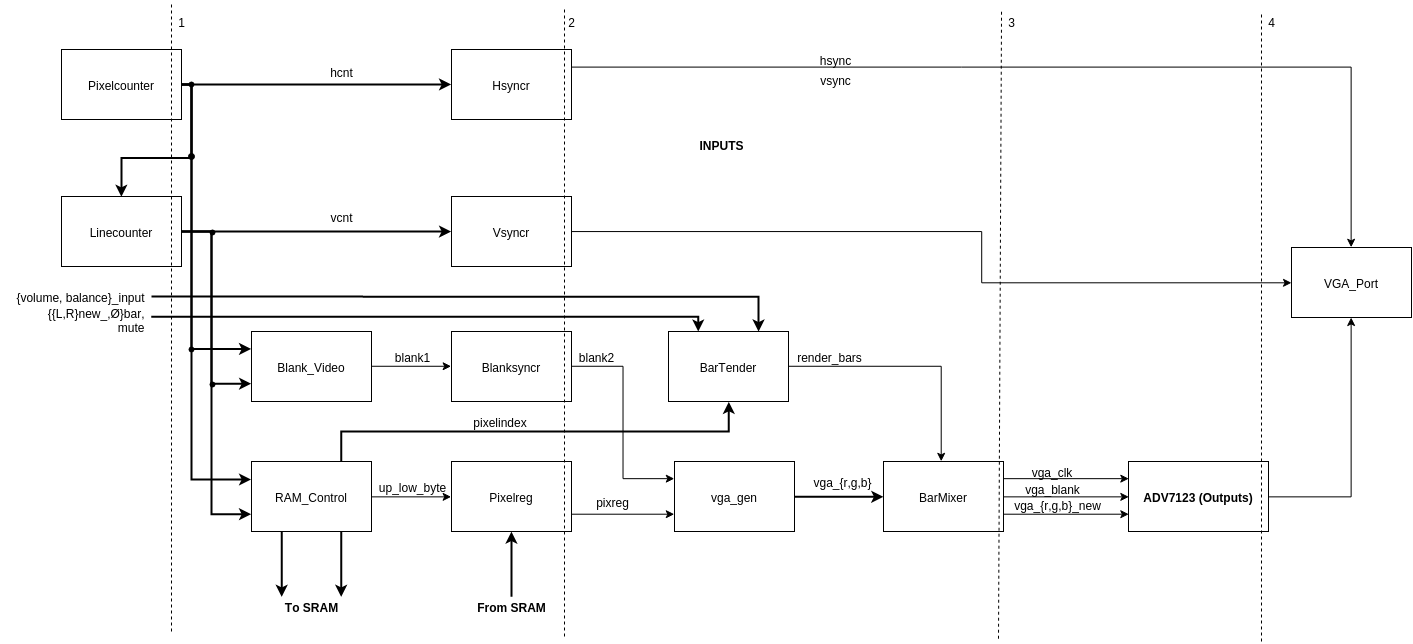
\includegraphics[scale=0.35]{vgadrive.png}
        \caption{Block diagram of vga\_drive}
        \label{fig:vgadrive}
\end{figure}

\begin{figure}[h]
        \caption{List of input signals}
        \label{tab:input}
\begin{tabular}{|r|l|}
        \hline
        \multicolumn{2}{|c|}{Input signals}\\
        \hline
        \multicolumn{1}{|c}{Name} & \multicolumn{1}{c|}{Description} \\
        \hline
        volume\_input & a 4 bit input containing volume information\\
        \cline{1-2}
        \hline
        balance\_input & a 4 bit input containing balance information\\
        \cline{1-2}    
        \hline
        bar & a n bit input containing signal sound input signal level\\
        \cline{1-2}    
        \hline
        new\_bar & a n bit input containing manipulated input signal level\\
        \cline{1-2}    
        \hline
\end{tabular}
\end{figure}

\begin{figure}[h]
        \caption{List of output signals}
        \label{tab:outputs}
\begin{tabular}{|r|l|}     
        \hline
        \multicolumn{2}{|c|}{output signals}\\
        \hline
        \multicolumn{1}{|c}{Name} & \multicolumn{1}{c|}{Description} \\
        \hline
        vga\_clk & clock signal needed for scanning\\
        \cline{1-2}
        \hline
        vga\_blank & a blanking signal for blanking when reseting scan\\
        \cline{1-2}    
        \hline
        vga\_(r,g,b) & three signals containing color information\\
        \cline{1-2}    
        \hline
\end{tabular}
\end{figure}

  \subsection{VGA\_driver:bartender}
  \subsection{VGA\_driver:barmixer}





\chapter{Challenges in the Design and Proposed Approach}\label{ch:challenges}
%\emph{Challenges in the Design and Proposed Approach (Main 2 or 3 challenges and proposed solutions, 1/2 to 1 page per challenge).}

%% Remove the text above

The major problem in the project is the merging of the different modules together
at top level. Most of the modules will be written and debugged separately and
only need minor adjustments before they have been used in a bigger system.
This puts high pressure on this document since a well thought through and described
design hopefully will result in pieces matching together.

A solution is to create and debug all modules and submodules individually
using test benches and waveforms to make sure the modules work exactly as
they are supposed to before putting them all together.

\section{The Logic of Adjusting Volume and Balance}
This is a challenge. It will be solved.


\section{Low Pass Filtering}
Different approaches to making a function for a low pass filter will be considered.

The low pass filter will be a part of the \verb=Analysis= module since it will only be used to refine the displayed power levels. The respective bars rendered on the screen will be delayed by at least 100 ms in order to allow a satisfactory result of the filtering, since there s a need for future values and the filtering is done in real time.

Before implementation, time will be put aside to study and understand the problem further.


\section{Bar Graph Rendering}
Stuff has to be rendered on the screen. This is not an issue, but rendering the right stuff is.



\chapter{User Interface}\label{ch:UI}
%\emph{User Interface (How to control the system + image visualized on the screen).}





The user interface will be able to desplay all the manageable settings on a VGA screen %	\\fotnot{req 3}.
	Ther will in total be four bars. One to indicate the left incomming power, one to indicate the right 
	incoming power, one to indicate the modified left power and one to incidate the modified right power.

	The user interface will also desplay the current volume graduated in dB. The scale goes form -15 dB to +15 dB.







%% Remove the text above


%\appendix
%\chapter{Appendix: System Overview}\label{app:overview}
%\pagenumbering{Roman}
%%\newpage
\begin{figure}[H]
  \centering
  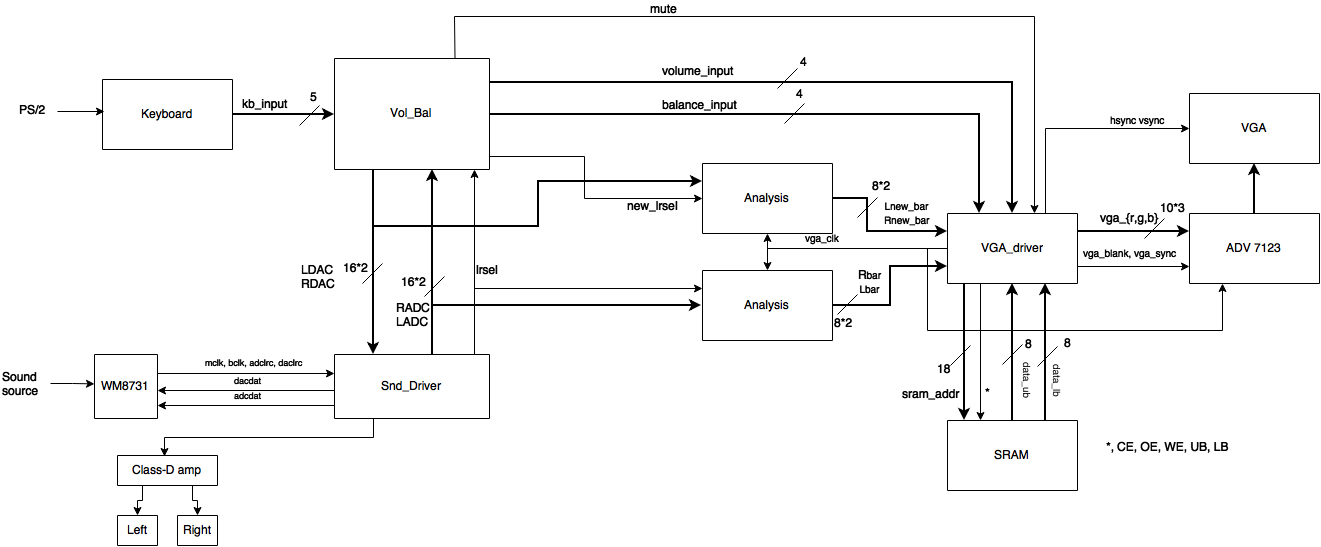
\includegraphics[angle=90, scale=.20]{overview}
%  \caption{This picture is to be redrawn to properly fit a paper layout.}
  \label{fig:hi_overview}
\end{figure}



\end{document}
